\documentclass[]{report}

% Include packages
\usepackage[utf8]{inputenc}
\usepackage[T1]{fontenc}
\usepackage[a4paper,width=150mm,top=25mm,bottom=25mm]{geometry}
\usepackage{fancyhdr}
\pagestyle{fancy}
\usepackage{graphicx}
\usepackage{listings}
\usepackage{amsmath,amsfonts,amssymb,amsthm}
\usepackage{bbm}
\usepackage[
backend=biber,
style=trad-plain,
sorting=ynt
]{biblatex}

\addbibresource{CRG.bib}

% Keywords command
\providecommand{\keywords}[1]
{
	\small	
	\textbf{\textit{Keywords---}} #1
}

% Font style for Python code inclusion
\lstset{frame=tb,
	language=python,
	aboveskip=3mm,
	belowskip=3mm,
	showstringspaces=false,
	columns=flexible,
	basicstyle={\small\ttfamily},
	numbers=none,
	numberstyle=\tiny\color{gray},
	keywordstyle=\color{blue},
	commentstyle=\color{dkgreen},
	stringstyle=\color{mauve},
	breaklines=true,
	breakatwhitespace=true,
	tabsize=3
}


% Title Page
\title{Customer Reviews: A Conditional Generative Model on the Basis of Clustered Text Data}
\author{Nils Gandlau, Jean Maccury, Fabian Ulmer \\
		\small Pattern Analysis and Machine Intelligence \\
		\small Goethe Universität Frankfurt}



\begin{document}
\maketitle


\begin{abstract}
	The goal of generative models is to find patterns in data, which can ultimately be recreated in a generated output. Recurrent Neural Networks (RNN) implementing a Long Short-Term Memory (LSTM) architecture have gained increasing popularity in this area, specifically in learning from and generating new text in accordance with the input data. In this project, our aim is to increase the influence one can take on the output of such a model. To this end, working with the Amazon Customer Review Dataset, we start by using novel Natural Language Processing techniques for feature extraction purposes. The resulting data is then clustered by means of an unsupervised Random Forest approach. Finally, we build a conditional model, consisting of multiple RNNs whose output will depend on the resulting cluster. The goal is to create a model which generates appropriate customer reviews based on the input it receives and the corresponding cluster.   \\\\
	This project serves as a final group submission for the course "Pattern Analysis and Machine Learning" at Goethe-University Frankfurt. \\\\
	\keywords{Natural Language Processing, Unsupervised Clustering, Recurrent Neural Network, LSTM, Text Generation, Customer Reviews}	
\end{abstract}

\tableofcontents

\chapter{Introduction}
Text generation can be understood as a task in which textual data is created according to specific rules or patterns. The goal herein usually lies in delivering constant satisfactory output, where the term "satisfactory" is not necessarily easy to define, let alone to measure. If, for instance, we try to generate Shakespearean poetry, we may seek to be able to fool a literary enthusiast with our results. Nowadays, good results can been achieved in this area using Machine Learning approaches, for example, Recurrent Neural Networks (RNNs)\cite{karpathy}. However, those models are often restrictive with regard to the control one can have over the output. When given a starting sequence, the model completes it with the most appropriate (i.e. probable) output based on what the model has learned. But what if we want to condition our output on more than a starting sequence? Our approach aims to give a more fine-tuned control over the generated content of the network by conditioning the RNN on subsets of the data. These subsets are defined by clusters they are comprised in, which are computed prior to the model setup. Those are consequently used to nudge the model towards a certain output. \\
Of course, we need to take into account that this type of task is usually of unsupervised nature. The textual input data is not split into classes, it is rather a corpus of texts which adhere to a single class. This also applies to our case, where the data consists of a set of customer reviews for products. Defining classes might be obvious: we could for example choose product types as our classes. Unfortunately, it is not always that simple. As for our choice, we prefer to include more factors in the clustering logic, which is why we employ an unsupervised clustering technique for our endeavor. \\
Therefore, it is necessary that we pre-process out data in a way that it can be clustered in a meaningful way. Fortunately, the field of Natural Language Processing provides numerous feature extraction techniques, which we make use of for our purposes. \\
As to the unsupervised clustering, we use a fairly uncommon approach that makes use of proximity values for data points, an inherent measure of the Random Forest Model. The implementation of this approach in Python, as well as the assessment of its usefulness as a method for unsupervised clustering is one of the goals of this project.


\chapter{Data}
The dataset that underlies our approach is the Amazon Customer Reviews Dataset \cite{amazondataset}, a dataset published by Amazon in which they have aggregated over 130M customer reviews with a set of features describing every single one. In the following part, we will take a look at the structure of this dataset, specifically the features that will be relevant to our project.

\chapter{Models, Tools and Frameworks}
\section{General}
In this section, we will describe the models, tools and frameworks we make use of in our project, starting with more general information and followed by details with regard to the different aspects our project can be broken into.\\

The application is programmed in Python 3 and the code is structured as a package. Python provides us with a set of well developed and documented Data Science libraries, as well as the Jupyter Notebook, which we use to run our code, comment it with markdown all the while visualizing our results in the same document.

\section{Text Analysis}

\section{Unsupervised Clustering}

\section{Text Generation}


\chapter{Text Analysis}

\chapter{Unsupervised Random Forest Clustering}
\section{Random Forest}
Random Forest is a supervised Machine Learning algorithm, developed by Leo Breiman in 2001 \cite{breiman2001}, which due to its straightforward implementation as well as robustness with regard to input data, has found extensive use in research and industry. The algorithm can be seen as an extension of the decision tree. The idea is to create an ensemble, i.e. a forest of decision trees. In other words, we want to combine numerous weak learners in order to improve our results. Decision trees are inherently susceptible to overfitting, especially deep decision trees, where the leaves end up simply reflecting very small subsets of the training data, resulting in failure to generalize on validation data. Random Forests overcome these weaknesses by building multiple trees using random subsets both of the data points and of the features. This increases the model variance, making overfitting less of an issue. \\


\section{Clustering}

Clustering can be described as the process of logically grouping data. While sometimes these groups may simply arise from the problem at hand, this is often not the case. What we then want is to find clusters that best fit our data and problem. This leads to numerous questions and choices, like the number of classes we want to define. In the context of Machine Learning, clustering is generally defined as a technique for unsupervised learning, as in supervised learning the clusters would be defined as the labels.\\

There exist innumerable approaches to tackle the many different issues one can encounter in this subject and we will look at the general aspects such an approach needs to cover. First, there is the need for a dissimilarity measure, in other words, a measure for how distinct two data points are. A commonly used measure is the squared Euclidean distance, it is even necessary for the K-Means algorithm. However, there can be settings where this distance measure is not well suited. In spaces of high dimension, the Euclidian distance between two data points starts becoming uniform, making it absolutely unsuitable as a distance measure \cite{distmetricsbehavior}.\\
Another aspect one has to consider is the number of clusters to be defined. The approach greatly depends on whether a predefined number has been set or not. Some algorithms, like again K-Means, work with a given number $K$ of clusters. It is however possible to take an iterative approach to find the most suitable amount of clusters. Still, some algorithms will not take $K$ as an input at all and build the clusters based on different arguments.
Finally, of course, one needs to choose an algorithm. In this context, what we can look at is the type of clustering algorithm. We are not going into too much depth, but the algorithms can be clustered (pun intended) according to the method they employ. K-Means is attributed to the partitioning algorithms, of which a defining feature is that the number of clusters is defined from the start, and also that the subsets are non-overlapping. Figure \ref{fig:clustermethodcomparison} displays the clustering results for different algorithms of different types. On the far left, we can see the partitioning algorithm K-Means. It becomes apparent that depending on the problem, the choice of the clustering algorithm can be of great importance.  \\
\begin{figure}[h]
	\centering
	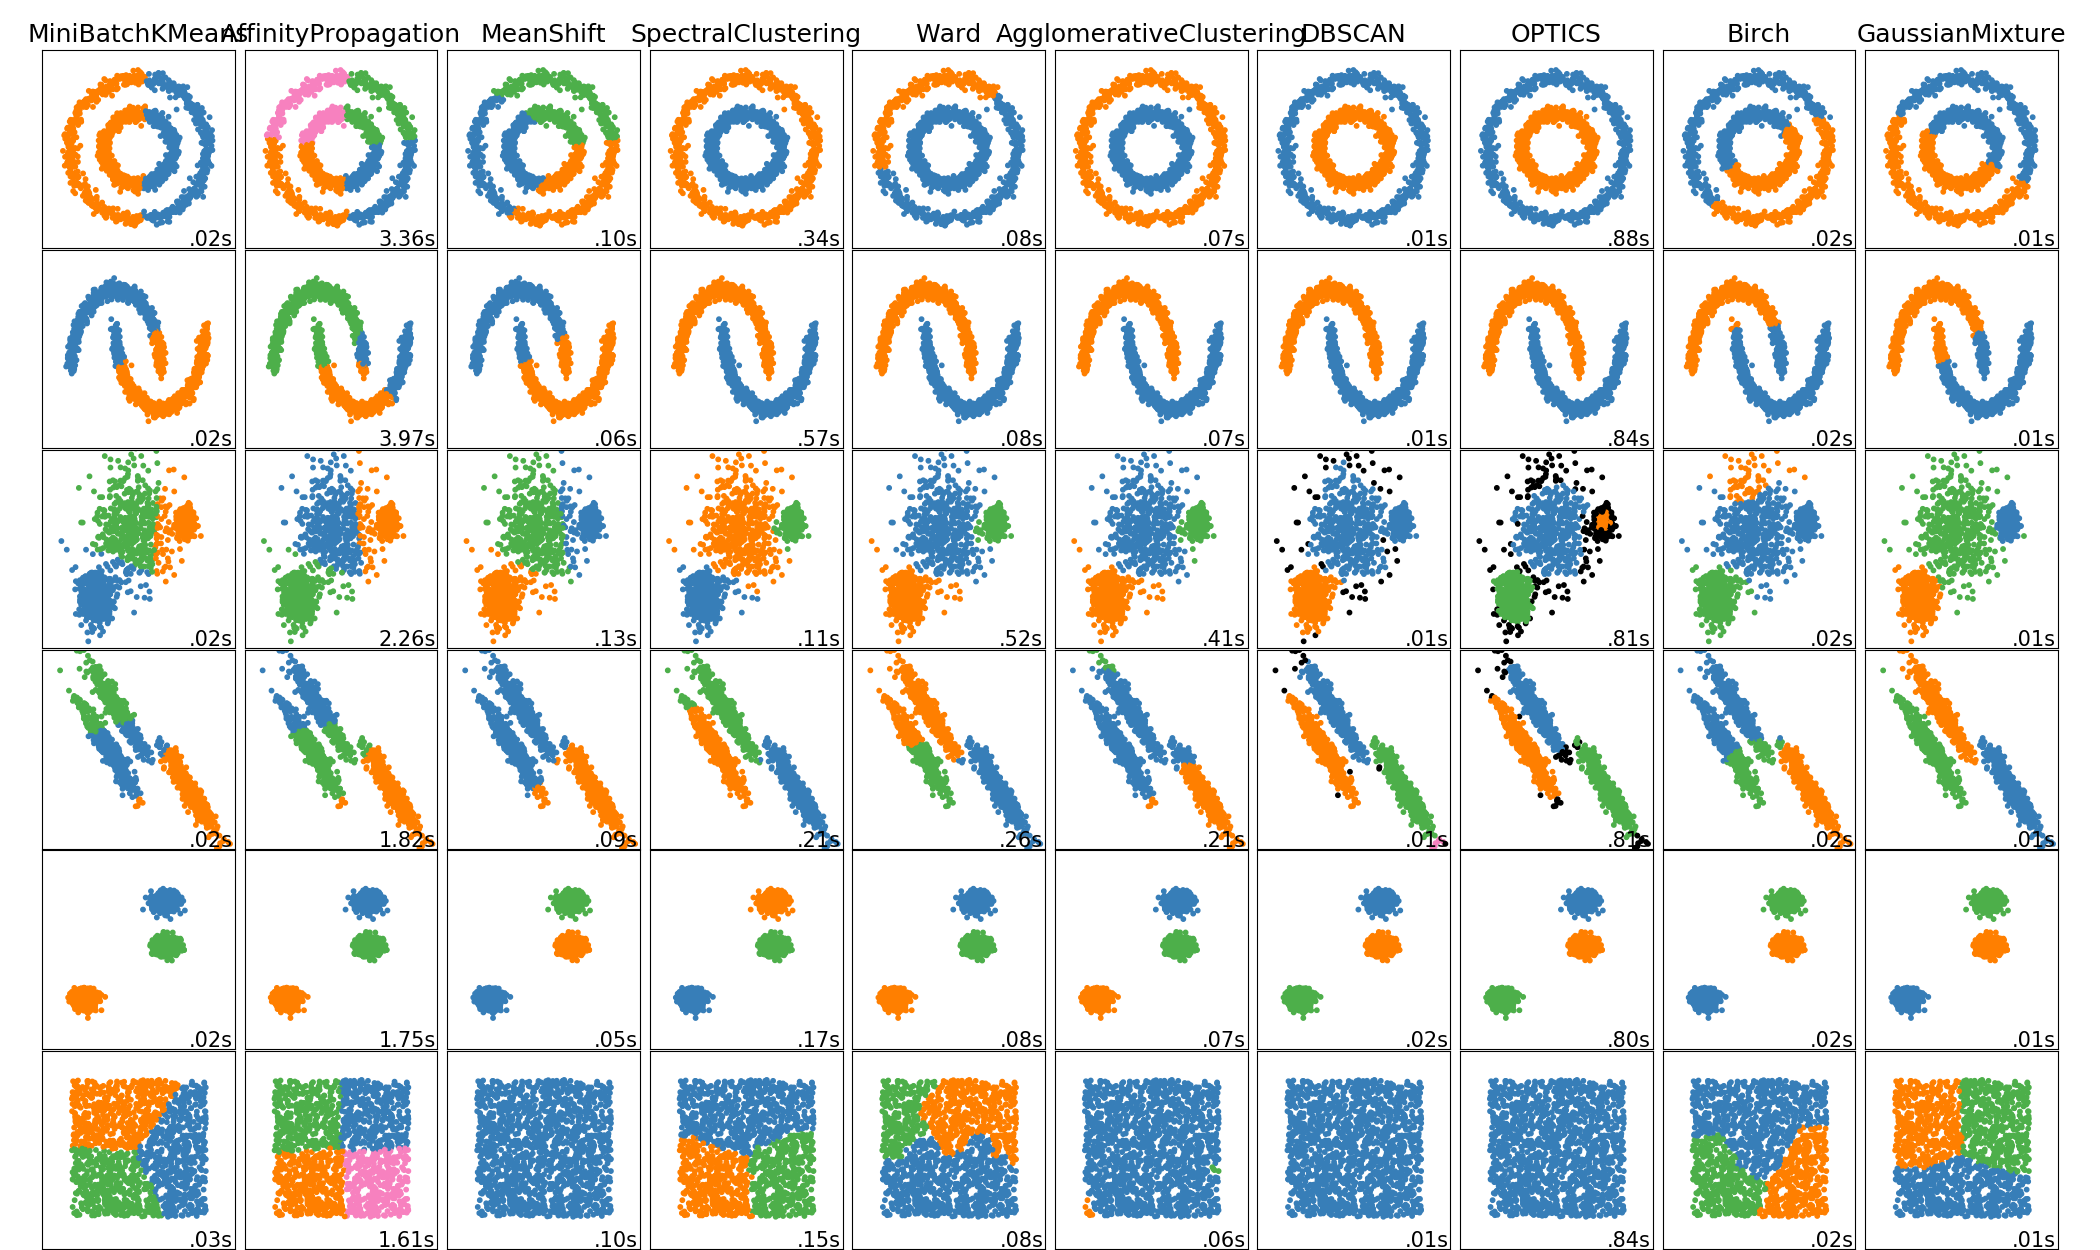
\includegraphics[width=0.7\linewidth]{Images/cluster_method_comparison}
	\caption[Clustering methods]{Clustering results of different algorithm.}
	\label{fig:clustermethodcomparison}
\end{figure}

Now, we are going to look at how the approach we have used in our project covers these aspects.


%TC:ignore
\printbibliography[title={References}]
%TC:endignore

\end{document}          
